\documentclass[10pt,a4paper,final]{article}
\usepackage[utf8]{inputenc}
\usepackage{amsmath}
\usepackage{graphicx}
\usepackage{amsfonts}
\usepackage{amssymb}
\usepackage{mcode}
\usepackage{hyperref}
\hypersetup{
    colorlinks,
    citecolor=black,
    filecolor=black,
    linkcolor=black,
    urlcolor=black
}
\author{Alessio Russo - alessior@kth.se (911103-T192) \\ Lars Lindemann - llindem@kth.se (891113-4131)}
\title{KTH - Royal Institute of Technology \\ \Large{Pattern Recognition (EQ2340) - Exercise Project }\\ A.1 - HMM Signal Source}
\begin{document}
\maketitle
\tableofcontents

\section{Exercise A 1.1}
All functions have been implemented in a sufficient way and can be found in the attached zip-file. It is important to mention that the function \textit{@DiscreteD/rand} has been extended, such that it is possible to use it not only for scalar features, but also for features with more than one dimension. The used \textit{isWhite} functionality will be explained additionally in the end of this report.
\newpage
\section{Exercise A 1.2}
In addition to the test file \textit{Assignment1Verification.m}, an additional function was implemented, \textit{isWhite}, in order to test the whiteness of a time series.
\subsection{Exercise A 1.2.1}
For this exercise the following data was used:
$$
A = 
 \begin{pmatrix}
  0.99 & 0.01 \\
  0.03 & 0.97
 \end{pmatrix} \quad
 \mathbf{q} = 
 \begin{pmatrix}
  0.75\\
  0.25
 \end{pmatrix} 
 \quad
 \mathbf{b} \sim
 \begin{pmatrix}
  \mathit{N}(0,1) \\
  \mathit{N}(0,4)
 \end{pmatrix} 
 $$
If $P(S_t=j)=const$ for all $t$, the following equation should hold:
$$\mathbf{p}=A^T \mathbf{p}$$
and one of the eigenvectors belonging to an eigenvalue with value $1$ should be equal to the initial state distribution. 
\\It turns out, that $A^T$ has one eigenvalue of $1$ with the normalised eigenvector ($0.9487$,$0.3162$), which is a scaled version of ($0.75$,$0.25$).
\\ \\
Another proof would be to calculate the probability:
$$P(S_t=j)=\sum_k P(S_t=j,S_{t-1}=k)=\sum_k P(S_t=j|S_{t-1}=k)P(S_{t-1}=k)$$
Which can be rewritten in the following compact notation $\mathbf{p}_t = A^T \mathbf{p}_{t-1}$, then for $t=1$:
$$\mathbf{p}_{1} = A^T \mathbf{q}$$
We find out that $\mathbf{p}_{1}= \mathbf{q} \Rightarrow \mathbf{p}_{2}=\mathbf{p}_{1}= \mathbf{q}$, etc....
\subsection{Exercise A 1.2.2}
Three experiments gave the following tuples of probabilities ($0.7843$,$0.2157$), ($0.7137$,$0.2863$) and ($0.7944$,$0.2056$). These numerical values are close to the state probability $\mathbf{q}$.
\subsection{Exercise A 1.2.3}
The creation of this HMM can be seen as a GMM, where the weights $0.75$ and $0.25$ are used, since the HMM is stationary. Hence, the pdf of the HMM is:
$$
f(x) = 0.75b_1(x) + 0.25b_2(x)$$
where the output distribution functions $b_1$ and $b_2$ are scalar, gaussian and independent. The solution of this problem is given in the course compendium on page 13. Using theses formulas, the mean and the variance of x can be obtained:
\begin{align*}
\mu  &= \int_{\mathbb{R}} \! xf(x) \, \mathrm{d}x= 0.75\mu_1 + 0.25\mu_2 = 0.75\\
\sigma^2  &=\int_{\mathbb{R}} \! (x-\mu)^2f(x) \, \mathrm{d}x=0.75\sigma_1^2+0.25\sigma_2^2+0.75(\mu_1-E[x])^2+0.25(\mu_2-E[x])^2 = 3.4375
\end{align*}
The alternative way mentioned in the problem formulation gives the same result and will be presented shortly:
\begin{align*}
E[X] &= E_S[E_X[X|S]]\\
\text{var}[X] &=E_S[\text{var}_X[X|S]]+\text{var}_S[E_X[X|S]]
\end{align*}
Here $S$ denotes the state of the Markov Chain and $X$ the actual output of the HMM. Using
\begin{align*}
\mu = E_X[X|S]= 
\begin{cases}
\mu_1, &\text{for S=1}\\
\mu_2, &\text{for S=2}
\end{cases}\\
\text{var}_X[X|S]=
\begin{cases}
\sigma_1^2, &\text{for S=1}\\
\sigma_2^2, &\text{for S=2}
\end{cases}
\end{align*}
we obtain
$$
E_S[E_X[X|S]] = \sum_i^2 p_i E_X[X|S=i] = p_1E_X[X|S=1]+p_2E_X[X|S=2]
$$
where $p_1 = 0.75$ and $p_2=0.25$. Furthermore this results in
\begin{align*}
E_S[\text{var}_X[X|S]] &= \sum_i^2 p_i \text{var}_X[X|S=i] = p_1\sigma_1^2+p_2\sigma_2^2\\
\text{var}_S[E_X[X|S]] &= \sum_i^2 p_i(E_X[X|S]-\mu)^2= p_1(\mu_1-\mu)^2+p_2(\mu_2-\mu)^2
\end{align*}
and finally in
$$
\text{var}[X] = p_1\sigma_1^2+p_2\sigma_2^2+p_1(\mu_1-\mu)^2+p_2(\mu_2-\mu)^2
$$
These results in the same formulas and numerical values as given above.\\
Repeating this experiment in Matlab, the resulting values have been ($0.8232$,$3.7656$), ($0.8263$,$3.6270$) and ($0.7627$,$3.4295$). These values are close to the ones calculated in the section above, so we can assume the results are correct.
\newpage
\subsection{Exercise A 1.2.4}

It is characteristic of the HMM to stay within a state for a long time, since the probability for this are: $$P_{S_t|S_{t-1}}(1|1)=0.99 \sim P_{S_t|S_{t-1}}(2|2)=0.97$$\\ Depending on state 1 or 2, the mean value is 0 or 3 respectively. That is why there are these jumps visible within the graph, switching from one state to another. Note also the difference in variance.	
A typical curve is shown in figure \ref{fig:A1}:
\begin{figure}[h]
		\centering
		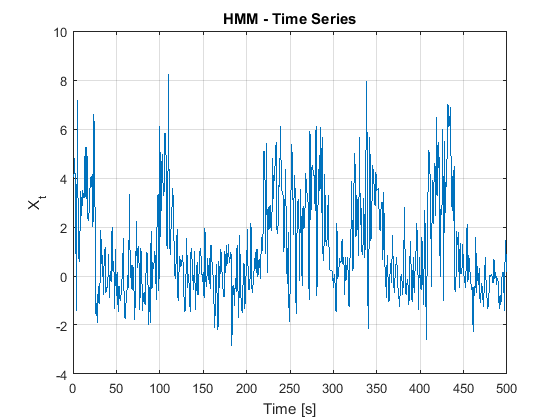
\includegraphics[width=0.55\linewidth]{./images/A1.png}
		\caption{HMM Sequence}
		\label{fig:A1}	
\end{figure}
The probability mass function is not a perfect Gaussian, therefore the spectrum of such time series, or the covariance, should not display the characteristics of a white noise signal.  \\
The covariance was analysed with the \textit{isWhite} function (section ~\ref{sec:iswhite}), which also shows whether the signal is white noise. 
\begin{figure}[h]
		\centering
		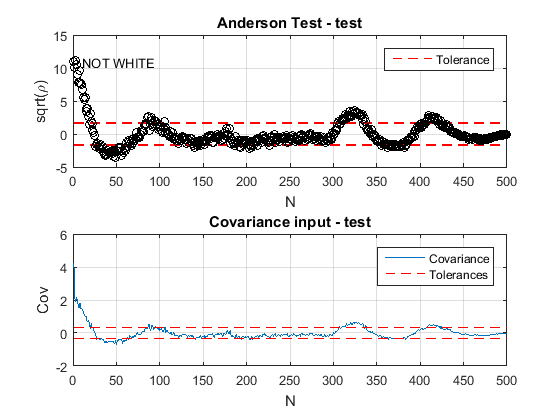
\includegraphics[width=0.55\linewidth]{./images/A2.png}
		\caption{Whiteness and covariance test of the HMM Sequence, tolerance is set to $10\%$.}
		\label{fig:A2}	
\end{figure}\\
In figure \ref{fig:A2} it is straightforward to see that the process has a complex correlation function that may be approximated by an ARMA process.
\newpage
\subsection{Exercise A 1.2.5}
A typical outcome of this HMM is shown in figure \ref{fig:A3}. The similarity is that the HMM stays within one state, using only one source, for a long time, because the A matrix has not changed. The difference is the mean shift for the second source, which makes it harder to distinguish between source 1 and 2. It is still possible to distinguish these signal by looking due to the different variance of the second source, still being not so high.
\begin{figure}[h]
		\centering
		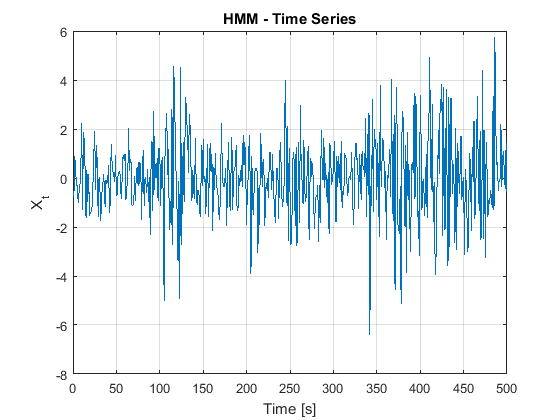
\includegraphics[width=0.55\linewidth]{./images/A3.png}
		\caption{Second HMM Sequence}
		\label{fig:A3}	
\end{figure}\\
Since the means are the same and the variance is not that high, and also due to the fact that the signal remains in one state for a long period of time the sequence looks like random white noise and a quick correlation analysis proves that, as seen in figure \ref{fig:A4}.
\begin{figure}[h]
		\centering
		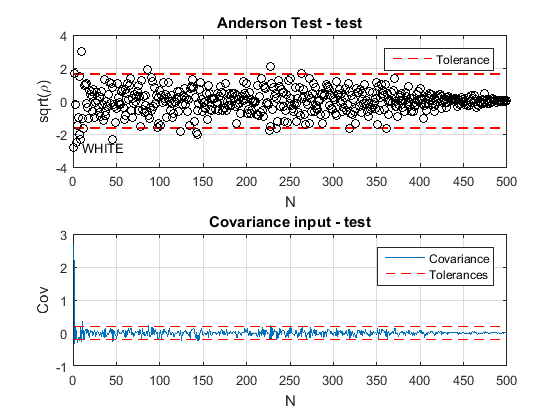
\includegraphics[width=0.55\linewidth]{./images/A4.png}
		\caption{Whiteness and covariance test of the second HMM Sequence, tolerance is set to $10\%$.}
		\label{fig:A4}	
\end{figure}
\newpage
\subsection{Exercise A 1.2.6}
A finite duration HMM is built by constructing a Markov Chain transition matrix with an additional column, which denotes the probability of transition to the exit node.
\\ In figure \ref{fig:A5} an finite duration HMM was created to generate $500$ samples, but after $4$ steps it transitions to the exit node.
\begin{figure}[h]
		\centering	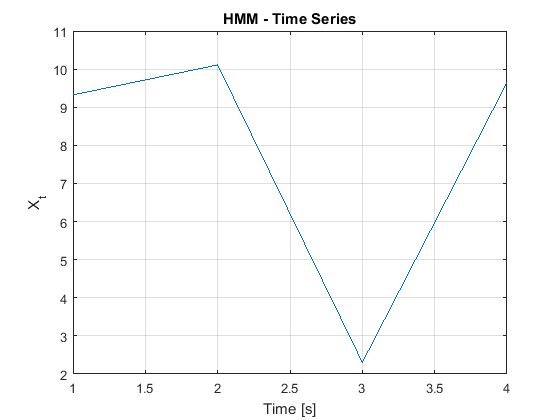
\includegraphics[width=0.55\linewidth]{./images/A5.png}
		\caption{Finite duration HMM}
		\label{fig:A5}	
\end{figure}\\
The code used is the following one:
\begin{lstlisting}
clear all; clc; close all;
q       = [0.75;0.25];
A       = [0.3, 0.1, 0.6; 0.1, 0.3, 0.6];
B(1)    = GaussD('Mean',1,'StDev',1);
B(2)    = GaussD('Mean',10,'StDev',2);
mc      = MarkovChain(q,A);
hHMM    = HMM(mc,B);
hashTable = zeros(20,1); %hashTable(i) represents the number of times 
						 %that the length of the sequence S was equal to i
for i=1:1000
    [X,S]       = rand(hHMM,500);
    hashTable(length(S)) =hashTable(length(S))+1;
end
disp(['Average: ' ]);
disp([num2str(hashTable(hashTable>0)./1000)]);
\end{lstlisting}
Which showed the following statistics:
\begin{lstlisting}
Average: 
0.608
0.231
0.097
...
\end{lstlisting}
$0.608\%$ is the percentual of times the sequence exited after the first state. It is correct since in the matrix $A$, for both the states, there is $60\%$ chance to exit the HMM directly.
\newpage
On the other hand the probability of exiting the HMM sequence after two steps is:
\begin{align*}
P(S_3=3)&=\sum_k P(S_3=3,S_{2}=k)=\sum_k P(S_3=3|S_{2}=k)P(S_{2}=k) \\
P(S_2=2)&=P(S_2=2|S_1=2)P(S_1=2)+P(S_2=2|S_1=1)P(S_1=1)\\
P(S_2=1)&=P(S_2=1|S_1=2)P(S_1=2)+P(S_2=1|S_1=1)P(S_1=1)
\end{align*}
Which is simply:
\begin{align*}
P(S_3=3)&=0.6(P(S_2=2)+P(S_2=1))\\
P(S_2=2)&=0.3\cdot 0.25+0.1\cdot 0.75=0.15\\
P(S_2=1)&=0.1\cdot 0.25+0.3\cdot 0.75=0.25
\end{align*}
Finally:
$$P(S_3=3)=0.6\cdot 0.4=0.24 \sim 0.231$$
We can say that the obtained results agree with the theoretical results.
\newpage
\subsection{Exercise A 1.2.7}
In this exercise the probability density functions are 2-D gaussians, so defined: 
 $$\mathbf{b} \sim
 \begin{pmatrix}
  \mathit{N}([0, 30],C_1) \\
  \mathit{N}([10, 55],C_2)
 \end{pmatrix} , \quad
 C_ 1=\begin{pmatrix}
  2 & 1 \\
  1 & 4
 \end{pmatrix}, \quad
 C_2 = \text{diag}(1,4)$$
 Therefore our output sequence is a matrix of size $2 \times T, T=500$, and it can be seen in figure \ref{fig:A6}. It is easy to distinguish between  the two Gaussian distributions when there is a state transition. 
\begin{figure}[h]
		\centering
		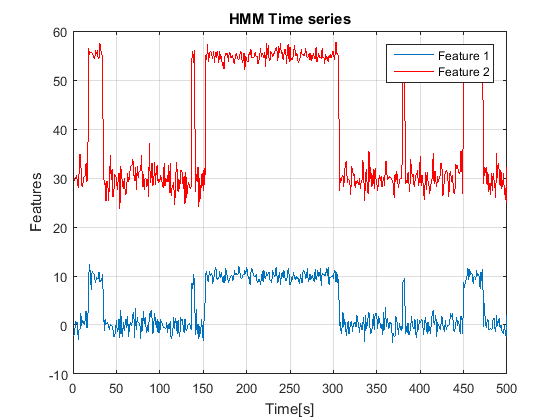
\includegraphics[width=0.55\linewidth]{./images/A6.png}
		\caption{HMM Sequence generated with bivariate Gaussians}
		\label{fig:A6}	
\end{figure}\\
The code used is the following one:
\begin{lstlisting}
q       = [0.75;0.25];
A       = [0.99 0.01;0.03 0.97];
B(1)    = GaussD('Mean',[0 30],'Covariance',[2 1;1 4]);
B(2)    = GaussD('Mean',[10 55],'StDev',[1 1]);
mc      = MarkovChain(q,A);
hHMM    = HMM(mc,B);
X       = rand(hHMM,500);
figure;
plot(X(1,:)) ;hold on; plot(X(2,:),'r') ;
legend('Feature 1','Feature 2');
xlabel('Time[s]');
ylabel('Features'); grid;
 \end{lstlisting}
\newpage
\subsection{isWhite function and Whiteness Test}\label{sec:iswhite}
This function was made in order to test the whiteness property of a signal $y_t$ and show the correlation function of that signal.
\\ \\ 
It is important to remember that a white noise signal has constant spectrum and covariance function $\gamma(t_1,t_2)=\gamma(\tau)=c$ for $t_1 = t_2, \tau=t_1-t_2$ (because of the stationarity), $0$ otherwise.
\\ \\
The whiteness property can be tested with the Anderson Whiteness Test, which is described below.\\
Suppose the signal $y_t=y(t)$ is white noise, then define:
$$\rho(\tau) = \frac{\gamma(\tau)}{\gamma(0)}$$
For a large number of observation of $y_t$, $N \gg 0$, $\rho$ has the following properties:
\begin{enumerate}
\item $\rho \sim N(0, \frac{1}{N})$.
\item $\rho(i)$ is uncorrelated to $\rho(j)$, %j \neq i $.
\end{enumerate}
Therefore $\sqrt{N}\rho(\tau) = \rho_N (\tau)\sim N(0,1)$.
\\ \\ 
The whiteness test procedure is the following one:
\begin{enumerate}
\item  Fix a confidence level $\alpha \in (0,1)$, preferably low.
\item Find $\beta$ such that $: P(|\rho_N| \leq \beta) = \alpha$.
\item Count the number of samples $\rho_N \in [-\beta, \beta]$ and call that number $n$.
\item If $\frac{n}{N} \leq \alpha$ then the test is passed and the signal is approximately white noise.
\end{enumerate}
\end{document}